% ******************************* PhD Thesis Template **************************
% Please have a look at the README.md file for info on how to use the template

\documentclass[a4paper,12pt,times,numbered,print,index]{Classes/PhDThesisPSnPDF}


% ******************************************************************************
% ******************************* Class Options ********************************
% *********************** See README for more details **************************
% ******************************************************************************

% `a4paper'(The University of Cambridge PhD thesis guidelines recommends a page
% size a4 - default option) or `a5paper': A5 Paper size is also allowed as per
% the Cambridge University Engineering Deparment guidelines for PhD thesis
%
% `11pt' or `12pt'(default): Font Size 10pt is NOT recommended by the University
% guidelines
%
% `oneside' or `twoside'(default): Printing double side (twoside) or single
% side.
%
% `print': Use `print' for print version with appropriate margins and page
% layout. Leaving the options field blank will activate Online version.
%
% `index': For index at the end of the thesis
%
% `draftclassic': For draft mode without loading any images (same as draft in book)
%
% `draft': Special draft mode with line numbers, images, and water mark with
% timestamp and custom text. Position of the text can also be modified.
%
% `abstract': To generate only the title page and abstract page with
% dissertation title and name, to submit to the Student Registry
%
% `chapter`: This option enables only the specified chapter and it's references
%  Useful for review and corrections.
%
% ************************* Custom Page Margins ********************************
%
% `custommargin`: Use `custommargin' in options to activate custom page margins,
% which can be defined in the preamble.tex. Custom margin will override
% print/online margin setup.
%
% *********************** Choosing the Fonts in Class Options ******************
%
% `times' : Times font with math support. (The Cambridge University guidelines
% recommend using times)
%
% `fourier': Utopia Font with Fourier Math font (Font has to be installed)
%            It's a free font.
%
% `customfont': Use `customfont' option in the document class and load the
% package in the preamble.tex
%
% default or leave empty: `Latin Modern' font will be loaded.
%
% ********************** Choosing the Bibliography style ***********************
%
% `authoryear': For author-year citation eg., Krishna (2013)
%
% `numbered': (Default Option) For numbered and sorted citation e.g., [1,5,2]
%
% `custombib': Define your own bibliography style in the `preamble.tex' file.
%              `\RequirePackage[square, sort, numbers, authoryear]{natbib}'.
%              This can be also used to load biblatex instead of natbib
%              (See Preamble)
%
% **************************** Choosing the Page Style *************************
%
% `default (leave empty)': For Page Numbers in Header (Left Even, Right Odd) and
% Chapter Name in Header (Right Even) and Section Name (Left Odd). Blank Footer.
%
% `PageStyleI': Chapter Name next & Page Number on Even Side (Left Even).
% Section Name & Page Number in Header on Odd Side (Right Odd). Footer is empty.
%
% `PageStyleII': Chapter Name on Even Side (Left Even) in Header. Section Number
% and Section Name in Header on Odd Side (Right Odd). Page numbering in footer

% Uncomment to change page style
%\pagestyle{PageStyleII}

% ********************************** Preamble **********************************
% Preamble: Contains packages and user-defined commands and settings
% ******************************************************************************
% ****************************** Custom Margin *********************************

% Add `custommargin' in the document class options to use this section
% Set {innerside margin / outerside margin / topmargin / bottom margin}  and
% other page dimensions
\ifsetCustomMargin
  \RequirePackage[left=37mm,right=30mm,top=35mm,bottom=30mm]{geometry}
  \setFancyHdr % To apply fancy header after geometry package is loaded
\fi

% Add spaces between paragraphs
%\setlength{\parskip}{0.5em}
% Ragged bottom avoids extra whitespaces between paragraphs
\raggedbottom
% To remove the excess top spacing for enumeration, list and description
%\usepackage{enumitem}
%\setlist[enumerate,itemize,description]{topsep=0em}

% *****************************************************************************
% ******************* Fonts (like different typewriter fonts etc.)*************

% Add `customfont' in the document class option to use this section

\ifsetCustomFont
  % Set your custom font here and use `customfont' in options. Leave empty to
  % load computer modern font (default LaTeX font).
  %\RequirePackage{helvet}

  % For use with XeLaTeX
  %  \setmainfont[
  %    Path              = ./libertine/opentype/,
  %    Extension         = .otf,
  %    UprightFont = LinLibertine_R,
  %    BoldFont = LinLibertine_RZ, % Linux Libertine O Regular Semibold
  %    ItalicFont = LinLibertine_RI,
  %    BoldItalicFont = LinLibertine_RZI, % Linux Libertine O Regular Semibold Italic
  %  ]
  %  {libertine}
  %  % load font from system font
  %  \newfontfamily\libertinesystemfont{Linux Libertine O}
\fi

% *****************************************************************************
% **************************** Custom Packages ********************************

% ************************* Algorithms and Pseudocode **************************

%\usepackage{algpseudocode}


% ********************Captions and Hyperreferencing / URL **********************

% Captions: This makes captions of figures use a boldfaced small font.
%\RequirePackage[small,bf]{caption}

\RequirePackage[labelsep=space,tableposition=top]{caption}
\renewcommand{\figurename}{Fig.} %to support older versions of captions.sty


% *************************** Graphics and figures *****************************

%\usepackage{rotating}
%\usepackage{wrapfig}
\usepackage{eurosym}

% Uncomment the following two lines to force Latex to place the figure.
% Use [H] when including graphics. Note 'H' instead of 'h'
%\usepackage{float}
%\restylefloat{figure}

% Subcaption package is also available in the sty folder you can use that by
% uncommenting the following line
% This is for people stuck with older versions of texlive
%\usepackage{sty/caption/subcaption}
\usepackage{subcaption}

% ********************************** Tables ************************************
\usepackage{booktabs} % For professional looking tables
\usepackage{multirow}
\usepackage{enumitem}

%\usepackage{multicol}
%\usepackage{longtable}
%\usepackage{tabularx}


% *********************************** SI Units *********************************
\usepackage{siunitx} % use this package module for SI units


% ******************************* Line Spacing *********************************

% Choose linespacing as appropriate. Default is one-half line spacing as per the
% University guidelines

% \doublespacing
% \onehalfspacing
% \singlespacing


% ************************ Formatting / Footnote *******************************

% Don't break enumeration (etc.) across pages in an ugly manner (default 10000)
%\clubpenalty=500
%\widowpenalty=500

%\usepackage[perpage]{footmisc} %Range of footnote options


% *****************************************************************************
% *************************** Bibliography  and References ********************

%\usepackage{cleveref} %Referencing without need to explicitly state fig /table

% Add `custombib' in the document class option to use this section
\ifuseCustomBib
   \RequirePackage[square, sort, numbers, authoryear]{natbib} % CustomBib

% If you would like to use biblatex for your reference management, as opposed to the default `natbibpackage` pass the option `custombib` in the document class. Comment out the previous line to make sure you don't load the natbib package. Uncomment the following lines and specify the location of references.bib file

\RequirePackage[backend=biber, style=numeric-comp, citestyle=numeric, sorting=nty, natbib=true]{biblatex}
\bibliography{References/references} %Location of references.bib only for biblatex

\fi

% changes the default name `Bibliography` -> `References'
\renewcommand{\bibname}{References}


% ******************************************************************************
% ************************* User Defined Commands ******************************
% ******************************************************************************

% *********** To change the name of Table of Contents / LOF and LOT ************

%\renewcommand{\contentsname}{My Table of Contents}
%\renewcommand{\listfigurename}{My List of Figures}
%\renewcommand{\listtablename}{My List of Tables}


% ********************** TOC depth and numbering depth *************************

\setcounter{secnumdepth}{2}
\setcounter{tocdepth}{2}


% ******************************* Nomenclature *********************************

% To change the name of the Nomenclature section, uncomment the following line

%\renewcommand{\nomname}{Symbols}


% ********************************* Appendix ***********************************

% The default value of both \appendixtocname and \appendixpagename is `Appendices'. These names can all be changed via:

%\renewcommand{\appendixtocname}{List of appendices}
%\renewcommand{\appendixname}{Appndx}

% *********************** Configure Draft Mode **********************************

% Uncomment to disable figures in `draft'
% \setkeys{Gin}{draft=true}  % set draft to false to enable figures in `draft'

% These options are active only during the draft mode
% Default text is "Draft"
% \SetDraftText{DRAFT}

% Default Watermark location is top. Location (top/bottom)
% \SetDraftWMPosition{bottom}

% Draft Version - default is v1.0
% \SetDraftVersion{v0.2}

% Draft Text grayscale value (should be between 0-black and 1-white)
% Default value is 0.75
%\SetDraftGrayScale{0.8}


% ******************************** Todo Notes **********************************
%% Uncomment the following lines to have todonotes.

\usepackage[colorinlistoftodos]{todonotes}
\newcommand{\mynote}[1]{\todo[author=kks32,size=\small,inline,color=green!40]{#1}}

% ******************************* Code Snippets ********************************
% \usepackage{fontspec}
% \newfontfamily\Consolas{Consolas}
% \lstset{basicstyle=\Consolas}
% \usepackage{listings}
% \usepackage{color}
\usepackage{fancyvrb}
\usepackage{multicol}
% \definecolor{commentcolor}{HTML}{999999}
% \definecolor{stringcolor}{HTML}{e6db74}
% \definecolor{backcolor}{HTML}{272822}
% \definecolor{keywordcolor}{HTML}{f92672}

% \lstdefinestyle{mystyle}{
%     aboveskip=3mm,
%     belowskip=3mm,
%     backgroundcolor=\color{backcolor},
%     commentstyle=\color{commentcolor},
%     keywordstyle=\color{keywordcolor},
%     numberstyle=\tiny\color{black},
%     stringstyle=\color{stringcolor},
%     basicstyle=\ttfamily\color{white},
%     breakatwhitespace=false,
%     breaklines=true,
%     captionpos=b,
%     keepspaces=true,
%     numbers=left,
%     numbersep=5pt,
%     showspaces=false,
%     showstringspaces=false,
%     showtabs=false,
%     tabsize=2,
%     sensitive=true
% }

% \lstset{style=mystyle}

% ************************ Thesis Information & Meta-data **********************
% Thesis title and author information, refernce file for biblatex
% ************************ Thesis Information & Meta-data **********************
%% The title of the thesis
\title{A rule-based geospatial reasoning system for trip price calculations}
%\texorpdfstring is used for PDF metadata. Usage:
%\texorpdfstring{LaTeX_Version}{PDF Version (non-latex)} eg.,
%\texorpdfstring{$sigma$}{sigma}

%% Subtitle (Optional)
\subtitle{}

%% The full name of the author
\author{Stefan Schenk}

%% Department (eg. Department of Engineering, Maths, Physics)
\dept{Department of Software Engineering}

%% University and Crest
\university{Amsterdam University of Applied Sciences}
% Crest minimum should be 30mm.
\crest{
\includegraphics[width=0.3\textwidth]{Hogeschool_van_amsterdam_logo_svg}}
%% Use this crest, if you are using the college crest
%% Crest long miminum should be 65mm
%\crest{
\includegraphics[width=0.45\textwidth]{University_Crest_Long}}

%% College shield [optional]
% Crest minimum should be 30mm.
%\collegeshield{
\includegraphics[width=0.2\textwidth]{CollegeShields/Kings}}


%% Supervisor (optional)
%% for multiple supervisors, append each supervisor with the \newline command
\supervisor{Willem Brouwer}

%% Supervisor Role (optional) - Supervisor (default) or advisor
% \supervisorrole{\textbf{Supervisors: }}
%% if no title is desired:
% \supervisorrole{}

%% Supervisor line width: required to align supervisors
%\supervisorlinewidth{0.35\textwidth}

%% Advisor (optional)
%% for multiple advisors, append each advisor with the \newline command
\advisor{Mewis Koeman}

%% Advisor Role (optional) - Advisor (default) or leave empty
% \advisorrole{Advisors: }
%% if no title is required
% \advisorrole{}

%% Advisor line width: required to align supervisors
%\advisorlinewidth{0.25\textwidth}


%% You can redefine the submission text:
% Default as per the University guidelines:
% ``This dissertation is submitted for the degree of''
%\renewcommand{\submissiontext}{change the default text here if needed}

%% Full title of the Degree
\degreetitle{Bachelor Software Engineering}

%% College affiliation (optional)
% \college{King's College}

%% Submission date
% Default is set as {\monthname[\the\month]\space\the\year}
%\degreedate{September 2014}

%% Meta information
\subject{Price Calculations} \keywords{{geospatial} {}}


% ***************************** Abstract Separate ******************************
% To printout only the titlepage and the abstract with the PhD title and the
% author name for submission to the Student Registry, use the `abstract' option in
% the document class.

\ifdefineAbstract
 \pagestyle{empty}
 \includeonly{Declaration/declaration, Abstract/abstract}
\fi

% ***************************** Chapter Mode ***********************************
% The chapter mode allows user to only print particular chapters with references
% Title, Contents, Frontmatter are disabled by default
% Useful option to review a particular chapter or to send it to supervisior.
% To use choose `chapter' option in the document class

% \includeonly{Chapter5/chapter5}

% ******************************** Front Matter ********************************
\begin{document}


\frontmatter

\maketitle
% \listoftodos


\begin{titlepage}

  \vspace*{\fill}
  \begin{center}
    {\Large A rule-based geospatial reasoning system for trip price calculations}
    \vspace{30pt}

    \textit{
      \begin{tabular}{ll}
        Author & Stefan Schenk, 500600679, +31638329419 \\
        Place and date & Medemblik, 10 Mar 2018 \\
        Educational Institution & Amsterdam University of Applied Sciences \\
        Department & HBO-ICT Software Engineering \\
        Supervisor & Willem Brouwer \\
        Company & taxiID, development team \\
        Company address & Overleek 4 \\
        & 1671 GD Medemblik \\
        & Netherlands \\
        Company Advisor & Mewis Koeman \\
        Period & 01 Feb 18 t/m 30 Jun 18
      \end{tabular}
    }
  \end{center}

  \vspace*{\fill}

\end{titlepage}
% ************************** Thesis Acknowledgements **************************

\begin{acknowledgements}

  Before you lies the graduation report that displays all the accomplishments and research conducted during the final phase of my Bachelor Software Engineering study at the Amsterdam University of Applied Sciences, written to fulfill the graduation requirements. The moment I was introduced to my assignment reminded me of a chapter in a book called Clean Code, in which this exact pursuit is used as a common example for which the book would provide solutions; “Now the two teams are in a race. The tiger team must build a new system that does everything that the old system does. Not only that, they have to keep up with the changes that are continuously being made to the old system. Management will not replace the old system until the new system can do everything that the old system does."~\citep{CleanCode}. This challenge, I could not have accomplished without the help of my colleques, therefore I would like to thank Dan Stefancu, Marco Strijker and Martin Zwaneveld for their insightful criticism that has led to the most useful lessons during my internship.

  Stefan Schenk

  Andijk, 01-05-2018

\end{acknowledgements}

% ************************** Thesis Abstract *****************************
% *CRITICAL: Do Not Use Symbols, Special Characters, Footnotes, or Math in Paper Title or Abstract.
%
% Use buzzwords
% Don't use jargon
% Generic to specific
% Pose questions
%
% In de samenvatting komt te staan:
% - Onderwerp-informatie;
% - probleemomschrijving/-analyse;
% - probleemvraag; - onderzoeksmethode;
% - de belangrijkste resultaten kort samengevat;
% - de (belangrijkste) conclusies.
%
\begin{abstract}

A purely geometrical interpretation of user-defined locations would allow taxi-companies around the world to set up rules so that trip prices could be calculated without depending on distinct postal code systems. Geolocation datatypes provide part of the solution, but the benifits of geometrical definitions are lost when areas intersect. A presidence hierarchy of rules that are tied to reusable locations would eliminate these competing rule matches.

A solution is proposed to implement a microservice with a single responsibility of calculating trip prices that is accessible to existing systems and portals in which users can define the pricing rules. The company for which this system is realized requires customers to be able to migrate to the new system without downtime, while keeping the existing rules that determine the prices of taxi trips.

The core system manages user and company data, this complicates identity management in the microservice. A JSON Web Token would allow user identity to be stored in the payload of the token, thereby delegating authentication to the core system, maintaining the single responsibility of the microservice.

\end{abstract}


% *********************** Adding TOC and List of Figures ***********************

\tableofcontents

% \printnomenclature[space] space can be set as 2em between symbol and description
%\printnomenclature[3em]

\printnomenclature

% ******************************** Main Matter *********************************
\mainmatter

%!TEX root = ../thesis.tex
%*******************************************************************************
%*********************************** First Chapter *****************************
%*******************************************************************************
\graphicspath{Chapter1/Figs/}

%%%%%%%%%%%%%%%%%%%%%%%%%%%%%%%%%%%%%%%%%%%%%%%%%%%%%%%%%%%%%%%%%%%%%%%%%%%%%%%%
% Introduction
%%%%%%%%%%%%%%%%%%%%%%%%%%%%%%%%%%%%%%%%%%%%%%%%%%%%%%%%%%%%%%%%%%%%%%%%%%%%%%%%
% - Introduction to the introduction
% - Context
% - Restatement of the problem
% - Restatement of the response
% - Roadmap
%
\chapter{Introduction}
Automatic fare estimations and calculations are one of many common features to go hand in hand with taxi dispatch systems. A potential passenger wants to book a ride using a mobile app by selecting the pickup and drop off locations, so that the app can display a list of available vehicles and corresponding prices. The passenger chooses the desired vehicle from the list, and a taxi arrives to take the passenger to the destination. When the destination is reached, the system calculates the final price, with or without discounts, including taxes, and additional costs added by the driver. Based on whether the passenger ordered a ride from the center of Amsterdam, or a desolate hard to reach location, the cost of such a trip can be higher or lower. For this reason, companies must be able to define prices based on locations so that the delivered work is still profitable. The project for which this thesis is written aims to improve the process of defining prices based on various factors, one of which is geographical locations.

%%%%%%%%%%%%%%%%%%%%%%%%%%%%%%%%%%%%%%%%%%%%%%%%%%%%%%%%%%%%%%%%%%%%%%%%%%%%%%%%
% Context
%%%%%%%%%%%%%%%%%%%%%%%%%%%%%%%%%%%%%%%%%%%%%%%%%%%%%%%%%%%%%%%%%%%%%%%%%%%%%%%%
% - General
% - Structure
% - Clients
%
\section{Context}
The company for which the project is realised is taxiID, an Amsterdam based company providing end-to-end cloud solutions for taxi companies. Founded as a startup that successfully introduced smartphone taxi booking in The Netherlands, and offers a wide range of IT solutions to serve the taxi market, including a passenger app, a driver app, administrative panels, and track and trace hardware. taxiID solutions have proven to be a reliable set of tools for all size businesses. For independent taxi companies with 2 cars or a companies with large fleets, affordable solutions are available. taxiID's goal is to deliver affordable, time-saving solutions for taxi companies to allow for convenient planning and dispatching without requiring local installation. Tough based in Amsterdam, the development team is located in Medemblik, consisting of two mobile developers, two backend developers, a designer and two project managers. Clients are located across the globe, introducing challenges when developing applications that rely on clearly defined locations and infrastructures that vastly differ between countries. YourDriverApp (YDA) is a light version of the original solution that is offered by taxiID more focussed on smaller taxi companies. Currently this label depends on services within taxiID to operate, which has to change in the near future.

%%%%%%%%%%%%%%%%%%%%%%%%%%%%%%%%%%%%%%%%%%%%%%%%%%%%%%%%%%%%%%%%%%%%%%%%%%%%%%%%
% Assignment
%%%%%%%%%%%%%%%%%%%%%%%%%%%%%%%%%%%%%%%%%%%%%%%%%%%%%%%%%%%%%%%%%%%%%%%%%%%%%%%%
% - Origin of the assignment
% - Description
% - Research question
% - Sub questions
%
% \section{Assignment}
% Waar gaat dit hoofdstuk over?
\section{Assignment}
% Waarom deze opdracht? Welke problemen moeten worden opgelost
YDA requires its own pricing calculation functionality that is similar to the existing taxiID implementation. All functionalities within the current system align with the clients demands, but some features introduce difficulties, for example: region names are too vague for specific database queries. A system must be implemented in which group admins can define pricing rules based on user defined locations and time schedules, that can be used for calculating a passengers trip price, or show prices of different products based on the trip the passenger is about to make. In the current system, locations are uploaded by taxi company group admins as excel sheets with departure and destination zip codes in conjunction with prices. This process works in countries with an unambiguous, explicit, well-defined postal code infrastructure. Postal codes are matched in efficient database queries, leaving less room for improvement in terms of performance. Interpretability is an issue however. Sheets may contain thousands of rows, making it hard to interpret and maintain. On top of that, countries without such systems are not covered by the functionality. There are two more types of pricing rules that cover the rest of trip pricing cases. A tier price system, that calculates fixed prices based cascading thresholds, and a dynamic pricing system that calculates prices per distance unit and minute. The term 'distance unit' is used on purpose, as distances are measured using different metrics in various countries. Pricing rules should be constrained by time frames, making rules available only for some hours a day, or only on christmas for example. Rules should be specifyable per product as different vehicle types have different prices, but are included in the same pricing rules. Discounts may be calculated with the trip price, and VAT should be displayed in the price breakdown. Some additional requirements to the system may be added in later phases, as Scrum is used to manage work iterations (this fact is covered later in this chapter). The system should be accessible to other systems, meaning that applications that currently rely on the old system should be able to migrate to the new system. As the old system shouldn't be used for new applications, as it was not designed for this use case. The system should have a single responsibility, and should be autonomous in that regard.

\section{Research}
% Hoe wordt dit onderzoek aangepakt?
% Designing research involves two separate sets of activities. The first involves determining everything you wish to achieve through the research project. This has to do with modelling the content of the research; we call this the con-ceptual design of a research project. The second set of activities concerns howto realise all this during the implementation stage of the project. This is called the technical research design.
Three main challenges that construct the assignment can be identified. Research must be done to attain the best possible way of mapping locations to pricing rules. What this means is that locations must be storable, comparable, and interpretable. The database must be able to store locations in an efficient manner, to which queries can be made as efficiently in order to find out whether a pricing rule applies to a given ride. For this to be the case, the stored locations must be comparable to the location of the passenger, or the destination. The user must be able to reason about his pricing rules, from which an understanding of his defined locations logically follows. But edge cases must be covered completely. For example, a rule in the current system dictates that a user traveling to Schiphol should receive a discount. But how would the system detect that this is the case? Or what if hotel guests receive discounts, but the neighbour shouldn't be allowed to use these discounts? Secondly, a system has to be developed that encapsulates the solution that is the result of the conducted research. It is helpful to extend the research of the problem to finding out how to incorporate the answers into a working system, where architecture has a major influence in the tools that are available. For example: if a solution to the main problem requires a database system capable of handling high quantities of geospatial queries, this requirement has to be satisfied in order to proceed in finding the final solution. Finally, a user interface has to be created that enables users to define the pricing rules. The complexity of the interface depends on how straight forward the price calculation system is put together. The user interface should also be available in multiple portals. The best way of making the systems capabilities available to the user through the UI in the portal, must be investigated. The UI must be built keeping the user in mind, simplifying complex rule management as much as possible.

\subsection{Questions}

From the description of the problem, one main important research question can be derived: \textit{How can a generic location-based price calculation system be implemented that could be used in every country?} \\

This question encapsulates the three important challenges that have to be dealt with before the project can successfully be implemented. In order to give a clear direction to the research, sub-questions are separated into three groups; location mapping, architecture and user interface.

\begin{enumerate}

	\item In what way can locations be represented to be universally interpretable?
	      \begin{enumerate}[label*=\arabic*.]
		      \item Which types of locations should be distinguished?
		      \item What are the main differences between postal systems used around the globe?
		      \item Can postal codes be abstracted to geospatial data while retaining the same usefulness in the system?
		      \item How can different types of locations be effectively stored in a database?
	      \end{enumerate}

	\item How could the price calculation system be integrated into the existing architecture?
	      \begin{enumerate}[label*=\arabic*.]
		      \item Which architectural patterns fit in with the exising architecture?
		      \item How will authentication be handled?
		      \item How is identity management handled?
	      \end{enumerate}

	\item How can a working system be realized while defining rules is as insightful as possible to the user?
	      \begin{enumerate}[label*=\arabic*.]
		      \item Which Database Management System (DBMS) is suited for this project?
		      \item Which views should exist, does a logical hierarchy exist among views?
		      \item How should locations be defined and managed by the user?
		      \item How should timeframes be handled in the interface?
	      \end{enumerate}

\end{enumerate}

The first group of questions is answered in the chapter \mynote{Add chapter name}. The second and third is answered in the chapter Proposed Approach. At that point, enough knowledge is available to implement a solution.

\section{Process}

A written working method is provided to the product owner, see Appendix \ref{appendix:pregame}, Pregame. The documents purpose is to clearly define the assignment and document the interpretation of the assignment definition so that miscommunications are found immediately. Requirements, scope and stakeholders of the project, as well as laying out the project timeline and estimated architecture based on use cases are clearly documented. Finally, a proposed solution is the result, which is agreed upon by the product owner before the backlog is created. Reading the document is recommended if more knowledge about the process and context of the assignment is desired.

%!TEX root = ../thesis.tex
%*******************************************************************************
%****************************** Second Chapter *********************************
%*******************************************************************************

\chapter{Encoding Locations}

\ifpdf
  \graphicspath{{Chapter2/Figs/Raster/}{Chapter2/Figs/PDF/}{Chapter2/Figs/}}
\else
  \graphicspath{{Chapter2/Figs/Vector/}{Chapter2/Figs/}}
\fi

\section{Introduction}
% Waar gaat dit hoofdstuk over?
To answer in what way locations can be represented to be universally interpretable, the definition of a location must be well understood. Encoding of locations has historically been of great importance, and is always being modernized. This chapter aims to find the best method of representing locations that is universally interpretable and most importantly usable in this project. GPS and Postal Codes are globally adopted and have proven to be reliable methods of encoding locations. Locations, plurally, suggesting that more than one location should be encoded. This is where the challenge lies.

\section{A Brief History Of Geographic Locations}

A location is roughly described as a place or position. Throughout history, various navigational techniques and tools like the sextant, nautical chart and marinner's compass were used, measuring the altitude of the North Star to determine the latitude $\phi$, in conjunction with a chronometer to determine the longitude $\lambda$ of a location on the Earth's surface.

\begin{figure}[htbp!]
  \centering
  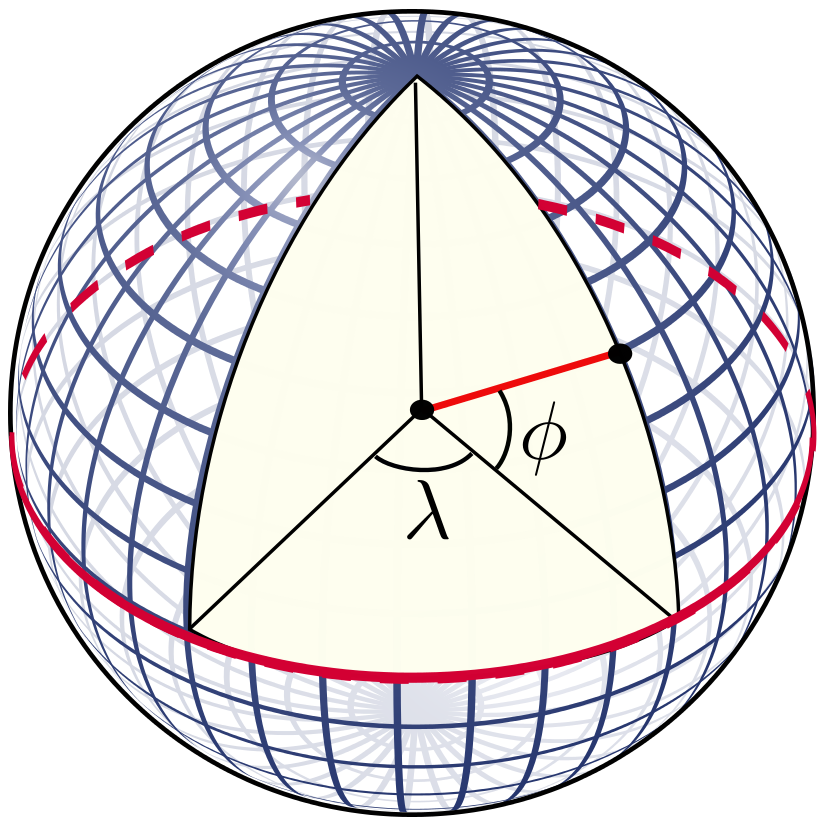
\includegraphics[width=.2\textwidth]{LatLngSphere}
  \caption[LatLngSphere]{A perspective view of the Earth showing how latitude and longitude are defined on a spherical model.}
  \label{fig:latlngsphere}
\end{figure}

Modern navigation relies on sattelites that are capable of providing information to determine a location with an accuracy of 9 meters. The precision of hybrid methods using cell towers and Wi-Fi Location Services enables precise tracking of modern devices. Latitude and longitude are often referred to as GPS coordinates, as GPS is often used to calculate latitude and longitude by receiving position and time code sequences from at least four sattelites. Addresses are another representation of a location used in navigation. Addresses are easier to communicate than a pair of GPS coordinates, but can be ambiguous, imprecise, inconsistent in format. Addresses commonly make use of Postal Code systems, which have reliably been assigned to geographical areas with the purpose of sorting mail. Although even today, there are countries that do not have a Postal Code system.
A location being roughly described as a place or position, can be decomposed as an abstract term to describe physical or imaginary areas with varying radiusses and shapes. You could prepend 'the location of' to the following terms as an example: America, the birthplace of Sokrates, Wall Street, the center of the universe, the Laryngeal Nerve of the Giraffe, churches in the Netherlands. The final example presents the main challenge of this project.

\section{Useful Location Types}

While setting up a backlog, a shared knowledge about the terminology used in the issues must be achieved. In the pregame document, the term "area" was defined as a collection of three or more coordinate pairs, or a collection of postal codes. A "point" was defined as one distinct coordinate pair or one distinct postal code. This way a location could either be an area or a point, with which all possibilities are covered. As stated in appendix \mynote{appendix pregame ref} definition of an area is precise, unambiguous and easy to use in compare in computer programs. A single point may match another single point if it’s the exact same point. A point may be sitting on top of a line or is contained within an area. The only other option is the negation of these statements. Because use cases for lines will be non-existent, points and areas are the proper candidates for spatial queries.

\section{Requisites of Locations}

A taxi company director wants to be able to set price or define discounts from or to a certain location. They would like to define prices based only on departure locations, or only on destination locations, or both. For example: 'to Schiphol, a trip should cost \euro 10,-', or 'from Falke hotels a trip should cost \euro 5,-', or 'from Falke hotels to Schiphol, the km price should be \euro 0,60'. In the current implementation, a record would be stored containing departure location, destination location and price for every combination, where locations were defined as zip codes. Instead, it would make sense to be able to reuse locations after they have been defined once.

\section{Literature Review}



In what way can locations be represented to be universally interpretable?
\begin{enumerate}
  \item Which types of locations should be distinguished?
  \item What are the main differences between postal systems used around the globe?
  \item Can postal codes be abstracted to geospatial data while retaining the same usefulness in the system?
  \item How can different types of locations be effectively stored in a database?
\end{enumerate}

%!TEX root = ../thesis.tex
%*******************************************************************************
%****************************** Third Chapter **********************************
%*******************************************************************************
\graphicspath{{Chapter3/Figs/Vector/}{Chapter3/Figs/}}

%%%%%%%%%%%%%%%%%%%%%%%%%%%%%%%%%%%%%%%%%%%%%%%%%%%%%%%%%%%%%%%%%%%%%%%%%%%%%%%%
% System Architecture
%%%%%%%%%%%%%%%%%%%%%%%%%%%%%%%%%%%%%%%%%%%%%%%%%%%%%%%%%%%%%%%%%%%%%%%%%%%%%%%%
% - What is most fitting solution to integrate TPS and UI into the
%   existing architecture?
%
\chapter{System Architecture}
\section{Introduction}
The family of systems that has formed through preceding architectural design decisions forms a collection of constrained connectors ready for new systems to assimilate. Flows of information are to be aligned with adjecent system components so that dependencies are satisfied, while making use of the most fitting technologies for great adaptation. Conventions, methods and styles throughout the technical and conceptual spectrums are applied, enabling the system architecture to evolve consistently at one pace. Additionally, adjecent systems are improved by solutions introduced in this chapter.

%%%%%%%%%%%%%%%%%%%%%%%%%%%%%%%%%%%%%%%%%%%%%%%%%%%%%%%%%%%%%%%%%%%%%%%%%%%%%%%%
% Architectural Patterns
%%%%%%%%%%%%%%%%%%%%%%%%%%%%%%%%%%%%%%%%%%%%%%%%%%%%%%%%%%%%%%%%%%%%%%%%%%%%%%%%
% - Which architectural patterns fit in with the exising architecture?
%
\section{Architectural Patterns}
The current system architecture consists of three API's and nine services that connect to four databases, as can be seen in Figure \ref{fig:Architecture}. They provide functionalities to portals and mobile apps. A separation exists between user interface, business logic and data storage that is known as the three-tier or multi-tier architecture, as described in \cite{IBM-3-tier}.

\begin{figure}[H]
	\centering
	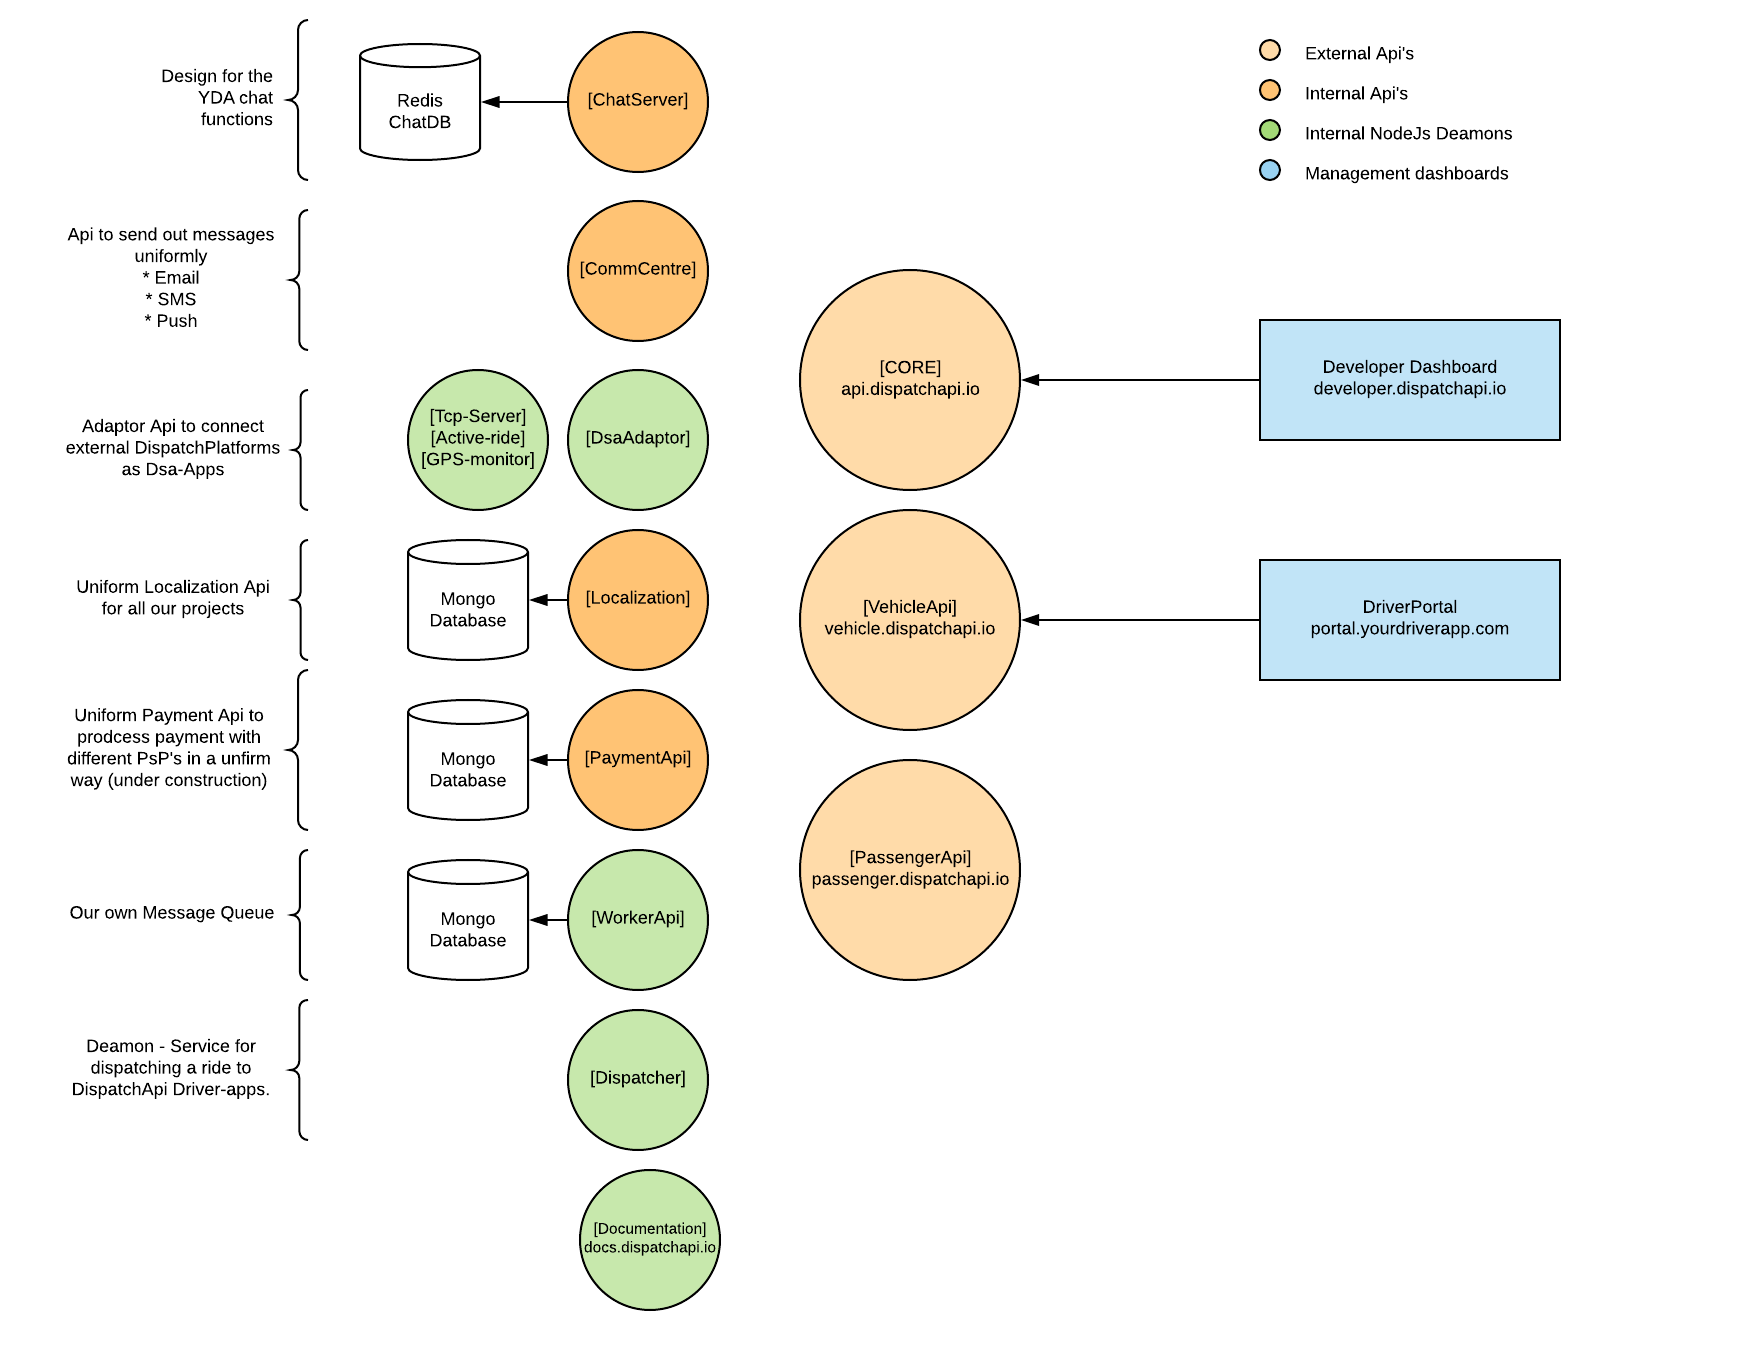
\includegraphics[width=1\textwidth]{Architecture}
	\caption[Current System Architecture]{Current System Architecture provided by taxiID.}
	\label{fig:Architecture}
\end{figure}

The bigger and smaller shapes in the Figure represent large API's and smaller services respectively. The orange colored services are used internally, the green shapes are used by external partners. The smaller services adhere to the pattern that is called service-oriented architecture, where application components provide services over a network typically.

\subsection{Monoliths}
The bigger shapes in Figure \ref{fig:Architecture} may be classified as monoliths.

% \[\mu ov \acute{o} \lambda \iota \theta o \sigma \qquad monolithos\]
\[Mo \nu \acute{o} \lambda \iota \theta o \varsigma \qquad monolithos\]
In the context of computer software, a monolithic system may have different definitions. Rod Stephens captures the meaning of a monolithic architecture quite broadly: "In a monolithic architecture, a single program does everything. It displays the user interface, accesses data, processes customer offers, prints invoices, launches missiles, and does whatever else the application needs to do" in \cite{rod-BSE}. In general, a monolith describes a software application which is designed without modularity. Even though the frontend is separated in some cases, it fits the description most accurately. Integration of TPS could be achieved by implementing TPS as a component of a monolith. But what logically follows is either duplication, or dependencies between large systems. The first contradicts an important principle of software engineering; don't repeat yourself (DRY), the second limits scalability and independence of deployment. The legacy system has demonstrated this issue because it has its price calculation system implemented in this manner, now facing difficulties providing the price calculation functionality to newer projects.

\subsection{Microservices}
% https://resources.sei.cmu.edu/asset_files/Presentation/2016_017_001_454683.pdf
If the previous price calculation system was implemented as a service, it could have been reused or redeployed as a second separate price calculation system for YDA instead. A consensual definition of microservices does not exist, but can be defined as a development technique that structures a system architecture as multiple loosely coupled services, exactly opposing the description of a monolith. The smaller shapes in Figure \ref{fig:Architecture} can be described as miniservices or microservices. Philipp Hauer describes the advantages of independent services accurately in \cite{microservices}, mentioning; improvements in development speed through parallel development, isolated deployment and continuous delivery (CD), scalability and potential parallelism, and independence in case of failure. Fair points of criticism have been made in regard to microservices. Jan Stenberg has pointed out that microservices are information barriers in \cite{JS-microservices}, meaning that the process of implementing a new system is degraded by the sense of ownership of specific services by developers. Technical downsides that have been discussed in general are: latency, testing, deployment, security, and message formats.

\subsection{Frontend and Backend}
A model-view-controller pattern is separating the business and presentation layers in various frontend projects. The requirements state that the frontend should be integrated in multiple portals. This would mean that separate views have to be developed for each portal, or the views should be provided to the portals via iframes. In the last case, it may be beneficial to combine the frontend and backend in the same project structure. However, this would be in conflict with this three-tier pattern, which is not desired in respect to the evolution of the system architecture. Integration of the backend would mean that the core system should contain the price calculation system as a component, and separation of the backend would mean that the backend would be set up as a separate service. Four possibilities may be listed as:

\begin{enumerate}
	\item Integrate views in existing portal, build TPS as a separate microservice
	\item Build separate service providing iframe views, build TPS as a separate microservice
	\item Integrate views in existing portal, integrate TPS as monolith component
	\item Build separate service providing iframe views, integrate TPS as monolith component
\end{enumerate}

The final decision is based on a more in-depth comparison, that can be found in table 4.1.1 in Appendix \ref{appendix:pregame}. An advice is given to separate the backend, and integrate the frontend. The final conclusion of Appendix \ref{appendix:pregame} states that the decision has to be made on a higher level, as many external factors play a role in the decision.

%%%%%%%%%%%%%%%%%%%%%%%%%%%%%%%%%%%%%%%%%%%%%%%%%%%%%%%%%%%%%%%%%%%%%%%%%%%%%%%%
% Information Dependencies
%%%%%%%%%%%%%%%%%%%%%%%%%%%%%%%%%%%%%%%%%%%%%%%%%%%%%%%%%%%%%%%%%%%%%%%%%%%%%%%%
%
\section{Information Dependencies}
The frontend separation or integration cases have little influence on the further design of the system. The backend separation case however, is only possible if information dependencies are met. This section lays out the information dependencies between systems. A conceptual model can be derived from the database schema design as found in Figure 4.7.1.1 of Appendix \ref{appendix:pregame}, having association and composition relations, see Figure \ref{fig:DataModel}.

\begin{figure}[H]
	\centering
	
\includegraphics[width=1\textwidth]{DataModel}
	\caption[DataModel]{Conceptual data model showing database entity relations.}
	\label{fig:DataModel}
\end{figure}

Figure \ref{fig:DataModel} will be used as reference throughout the upcoming chapters. In isolation, this model contains all the required information to calculate a price, given the parameters shown in Listing \ref{lst:request}.

\begin{lstlisting}[caption={Minimal external information required for a trip price calculation.}, label={lst:request}]
	{
		"companyId": string
		"daAppInstallId": string,
		"vehicleTypes": string[],
		"passengerCount": number,
		"requestedDate": ISODate,
		"departure": { "gps": { "lat": string, "lng": string } },
		"destination": { "gps": { "lat": string, "lng": string } }
	}
\end{lstlisting}

A user is identified by a combination of two identifiers: companyId and daAppInstallId. Assuming that companyId and daAppInstallId are provided in the authentication headers, the user can be identified. But this identity is futile if no pricing data is associated with it. There are two options with regard to storing the data in a way that user identity can be used to associate pricing information:

\begin{enumerate}
	\item A single shared database
	\item Multiple synchronized databases
\end{enumerate}

The first option allows TPS to have access to all neccesary data by default. The second option requires systems to drill changes down to depending systems.

\begin{figure}[H]
	\centering
	
\includegraphics[width=0.6\textwidth]{DataSync}
	\caption[DataSync]{Flow of data requests.}
	\label{fig:DataSync}
\end{figure}

If a company is added to the core system for example, the same company must be added to the TPS database. Multiple proposal were made aiming to solve the combination of authentication, authorization and data consistency problems. The next section expands on the accepted solution.

%%%%%%%%%%%%%%%%%%%%%%%%%%%%%%%%%%%%%%%%%%%%%%%%%%%%%%%%%%%%%%%%%%%%%%%%%%%%%%%%
% Authentication and Authorization
%%%%%%%%%%%%%%%%%%%%%%%%%%%%%%%%%%%%%%%%%%%%%%%%%%%%%%%%%%%%%%%%%%%%%%%%%%%%%%%%
% - How can authentication between services be implemented or improved?
%
\section{Authentication and Authorization}
In the legacy system, authorization was achieved by sending extra headers for each crucial piece of information, this is clarified in Appendix \ref{appendix:pregame}, chapter 3.4. To prevent duplication, the microservice could be connected to the database that is used by the core system, as example one in Appendix \ref{appendix:slides_2_authentication} suggests. But this makes the microservice less decoupled, and directly contradicts the desire to separate data dependencies. Appendix \ref{appendix:slides_2_authentication} lists four proposals that aim to solve this problem, from which the third option is accepted, as shown in Figure \ref{fig:Authentication}.

\begin{figure}[H]
	\centering
	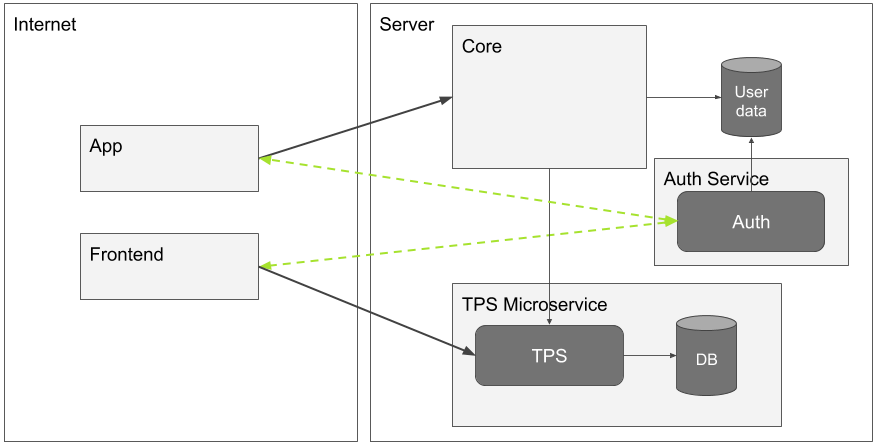
\includegraphics[width=1\textwidth]{Authentication}
	\caption[Authentication]{Accepted authentication proposal.}
	\label{fig:Authentication}
\end{figure}

The solution completely decouples the information requirements by keeping Core data and TPS data in their respective databases separated. A single directional flow of data to TPS ensures that the Core system remains the single source of truth. This accepted proposal is based on three other separate proposals, that will be explained in the upcoming subsections: OAuth 2.0 Proposal, JSON Web Token Proposal, and API Gateway Proposal. Only JSON Web Tokens were implemented, solving the problem of synchronizing user identity.

\subsection{Proposal OAuth 2.0}
This proposal delegates managing user identity to a separate authentication service that, similar to the pricing microservice, has its own single task of authenticating users. OAuth 2.0 is a protocol that has been designed to allow third-party apps to grant access to an HTTP service on behalf of the resource owner. This behaviour could be utilized to allow users to make use of services within the architecture, controlled by a single service, stored in a single token. A proposal was made in the Pregame document to combine oAuth with JWT and an API Gateway to introduce an automated authentication flow with a single token, instead of sending multiple headers, see Appendix \ref{appendix:pregame}.

\begin{figure}[H]
	\centering
	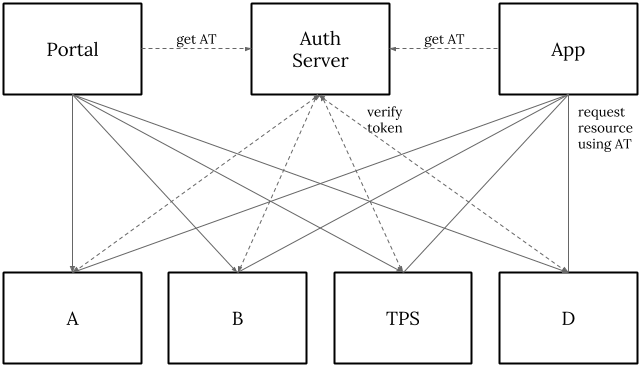
\includegraphics[width=.7\textwidth]{Auth1}
	\caption[OAuth 2.0]{OAuth requests where tokens are verified by Auth Server}
	\label{fig:Auth1}
\end{figure}

\subsection{Proposal JSON Web Token}
This proposal entirely removes the database connection to any user data. This is possible when a JSON Web Token (JWT) is used. A JWT may be signed with a cryptographic algorithm or even a public/private key pair using RSA. After the user enters valid credentials, the core system validates the credentials by comparing them with user data in the database.

\begin{lstlisting}[caption={Two user identifiers and registered claim names stored inside the payload of a JSON web token.}, label={lst:payload}]
	{
		"companyId": "59ea0846f1fea03858e16311",
		"daAppInstallId": "599d39b67c4cae5f11475e93",
		"iat": 1521729818,
		"exp": 1521816218,
		"aud": "tps.dispatchapi.io",
		"iss": "api.dispatchapi.io",
		"sub": "getPrices"
	}
\end{lstlisting}

The core system signs a token that with a secret that is known by the microservice. The token consists of three parts, separated by a fullstop. The first part (header) of the token contains information about the hashing algorithm that was used to encrypt the payload. This part is Base64Url encoded. The payload itself contains information stored in JSON format as shown in Listing \ref{lst:payload}. The identity of the user is stored in the payload that can only be revealed by whoever holds the secret with which it was signed. Then the message can be verified using the third part of the token, which is the signature. The verification step prevents tampering with the payload. Claims can be added to the payload as shown in \ref{lst:payload} to provide information about the token, as explained in \cite{JWT}.

\begin{figure}[H]
	\centering
	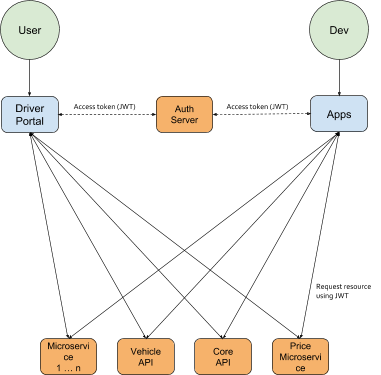
\includegraphics[width=.7\textwidth]{Auth2}
	\caption[Stateless JWT]{OAuth with stateless JWT token requests}
	\label{fig:Auth2}
\end{figure}

\subsection{Proposal API Gateway}
The final proposal allows services to be used by external agents is the API Gateway. It allows for a central middleware in which authentication and authorization is handled, where the microservices are shielded from public access, and all communication is established through the API Gateway \cite{api-gateway}. Next to authentication, the gateway could optimize the endpoints so that no multiple requests are needed from external agents to gather different types of resources. These calls could be made internally to the microservices behind the gateway. This also opens the possibility the freely change the microservices without changing the public endpoints exposed by the gateway, and even offers slow or instant transitions to different versions of microservices. The different proposals explain the improvements they may bring over some system. But the advice given is not tied to this project, instead to the entire Dispatch API. It’s advised to have a constructive dialogue about the future of the company, and the way it’s planning to scale. One could put a API Gateway in front of a monolithic app to help with transitioning to a microservice-oriented app.

\begin{figure}[H]
	\centering
	
\includegraphics[width=.7\textwidth]{Auth3}
	\caption[API Gateway]{API Gateway}
	\label{fig:Auth3}
\end{figure}

\subsection{Reflection}

%%%%%%%%%%%%%%%%%%%%%%%%%%%%%%%%%%%%%%%%%%%%%%%%%%%%%%%%%%%%%%%%%%%%%%%%%%%%%%%%
% Languages
%%%%%%%%%%%%%%%%%%%%%%%%%%%%%%%%%%%%%%%%%%%%%%%%%%%%%%%%%%%%%%%%%%%%%%%%%%%%%%%%
%
\section{Languages}
PHP
Typescript
Java

%%%%%%%%%%%%%%%%%%%%%%%%%%%%%%%%%%%%%%%%%%%%%%%%%%%%%%%%%%%%%%%%%%%%%%%%%%%%%%%%
% Frameworks
%%%%%%%%%%%%%%%%%%%%%%%%%%%%%%%%%%%%%%%%%%%%%%%%%%%%%%%%%%%%%%%%%%%%%%%%%%%%%%%%
%
\section{Frameworks}
Loopback
NodeJS
GraphQL

An important choice that has to be made is the framework in which the project is going to be built. The team has experience with LoopBack 3.0 \cite{lb}, but considering the fact that this microservice is very small, and may not need the large amount of abstractions, Express.js is more suitable for the job. Although this means that required functionalities, that come out of the box with Loopback, have to be replaced. The API should be capable of exposing endpoints (that are going to be specified in more detail in the next phase) that are available to the DriverPortal and to external services. The endpoints for the DriverPortal should expose CRUD operations on resources that are used to calculate a trip. The endpoint for external services has only one task, given some trip information, a price has to be calculated based on the rules of the application that has been used. As mentioned, the team has experience with Loopback, and having most code written in Loopback, making it easier to transfer pieces of functionality between projects. It has a built in ORM including CRUD endpoints. On the other hand, Loopback has a steeper learning curve, stagnating velocity among external or new developers. Keeping the code base up to date may be harder because of increased amount of dependencies. There’s no clear winner. The best choice should be the result of a consensus between core developers.

The backend should be loosely coupled, but should be accessible by all users who are able to authenticate and authorize themselves. It’s advised to implement the system as a microservice, because it separates the concern effectively. By implementing the system as a module, the implementation is entirely dependent on the existing system it’s implemented in, stalling modernization of architecture in the long run. The solution that is presented in the pregame solves this challenge by having one microservice handle the requests that are in some cases routed through the DispatchAPI. The requests sent by a user from any portal should be directed at the microservice, while price calculation requests should be routed through the DispatchAPI. Loopback should be used as a framework, preferably in combination with typescript.

Angular

The first non-functional requirement states that the solution should be seamlessly integrated in the portal. On top of that, a user shouldn’t have to log in again to make use of the pricing service from within that portal. Iframes, objects and embeds have been mentioned as potential solutions to integrate a frontend in several distinct portals. This problem affects more than just the pricing project, therefore a decision must be made on a higher level before the frontend will be integrated, but the decision is not required for the first sprint to start. The options that are available are: an integrated view inside the existing DispatchAPI project or a separate solution built in Vue2 with a material design style that can be integrated using an iframe. The user interface will contain an overview showing the main concepts that a user has to maintain: pricing rules, locations, discounts. The UI should be focussed on linear navigation with overviews of detail pages. The UI will contain a screen to assign rules and discounts to DaAppInstallations and debtors, a screen to define locations, a screen to edit rules, a screen to modify vehicle types, and a screen to define timeframes.

%%%%%%%%%%%%%%%%%%%%%%%%%%%%%%%%%%%%%%%%%%%%%%%%%%%%%%%%%%%%%%%%%%%%%%%%%%%%%%%%
% Databases
%%%%%%%%%%%%%%%%%%%%%%%%%%%%%%%%%%%%%%%%%%%%%%%%%%%%%%%%%%%%%%%%%%%%%%%%%%%%%%%%
%
\section{Databases}
MySQL
MariaDB
MongoDB

MongoDB should be used over an SQL database because of its scalability. MongoDB supports geographical location types, geospatial queries including the predicate to check which polygons contain a single point, or retrieving all points contained within a single polygon.

%%%%%%%%%%%%%%%%%%%%%%%%%%%%%%%%%%%%%%%%%%%%%%%%%%%%%%%%%%%%%%%%%%%%%%%%%%%%%%%%
% Paradigms
%%%%%%%%%%%%%%%%%%%%%%%%%%%%%%%%%%%%%%%%%%%%%%%%%%%%%%%%%%%%%%%%%%%%%%%%%%%%%%%%
%
\section{Paradigms}
The object-oriented programming (OOP) paradigm offers many ways to keep a system structured. Good software design has low coupling and high cohesion, meaning that software components should have a high degree of belongingness, and a low degree of dependence in respect of eachother.

As stated in the previous chapter, another paradigm that could potentially improve the price calculation system is called: functional programming (FP).

These two paradigms together are capable of providing a modular system that is highly cohesive, and very low coupled. To understand more about the structure of the system, a class diagram visualizes the most important components in \ref{fig:ClassDiagram}.

%%%%%%%%%%%%%%%%%%%%%%%%%%%%%%%%%%%%%%%%%%%%%%%%%%%%%%%%%%%%%%%%%%%%%%%%%%%%%%%%
% Tests
%%%%%%%%%%%%%%%%%%%%%%%%%%%%%%%%%%%%%%%%%%%%%%%%%%%%%%%%%%%%%%%%%%%%%%%%%%%%%%%%
%
\section{Tests}
Mocha
Chai

%%%%%%%%%%%%%%%%%%%%%%%%%%%%%%%%%%%%%%%%%%%%%%%%%%%%%%%%%%%%%%%%%%%%%%%%%%%%%%%%
% Software Validation
%%%%%%%%%%%%%%%%%%%%%%%%%%%%%%%%%%%%%%%%%%%%%%%%%%%%%%%%%%%%%%%%%%%%%%%%%%%%%%%%
%
\section{Software Validation}

Linting is the process of running a program that will analyse code for potential errors.

Sonarqube

Buddy-Works

CircleCI

Software Reliability is defined as the probability of an item to perform a required function under stated conditions for a specified period of time. New features often introduce bugs by adding functionalities that are broken, although the reliability of the existing functionalities may also be impacted because of changes in the existing code. To prevent units of code from malfunctioning, regression tests may be implemented to validate whether a unit still functions according to a set of conditions. Static and dynamic tests may be performed using the framework Mocha \cite{mocha} and the assertion library Chai \cite{chai}. To further reduce the chances of introducing bugs, some additional techniques could be used.

%%%%%%%%%%%%%%%%%%%%%%%%%%%%%%%%%%%%%%%%%%%%%%%%%%%%%%%%%%%%%%%%%%%%%%%%%%%%%%%%
% Conclusion
%%%%%%%%%%%%%%%%%%%%%%%%%%%%%%%%%%%%%%%%%%%%%%%%%%%%%%%%%%%%%%%%%%%%%%%%%%%%%%%%
% - Which decisions could be made following the research in this chapter?
%
\section{Premise}

integration vs separation frontend
integration vs separation backend




Taking all the different aspects in this chapter into account, the advised architectural design of TPS comprises of integrated frontend views in each required portal using the associated available technologies, a separate NodeJS microservice with its own MongoDB database, Loopback as a framework to quickly implement functionalities using Typescript and a combination of OOP and FP, authentication via JWT, automated tests using mocha and chai, and continuous delivery and automated testing using Buddy-Works.

\begin{table}[htbp!]
	\centering
	\begin{tabular}{c|c|c}
		\toprule
		& MySQL & MongoDB \\
		\midrule
		Point & \checkmark & \checkmark \\
		Polygon & \checkmark & \checkmark \\
		MultiPolygon & \checkmark & \checkmark \\
		MultiPolygon & \checkmark & \checkmark \\
		MultiPolygon & \checkmark & \checkmark \\
		MultiPolygon & \checkmark & \checkmark \\
		Intersect & \checkmark & \checkmark \\
		\bottomrule
	\end{tabular}
	\caption[Databases]{Required database features.}
	\label{tab:databases}
\end{table}
%!TEX root = ../thesis.tex
%*******************************************************************************
%****************************** Fourth Chapter *********************************
%*******************************************************************************
\graphicspath{{Chapter4/Figs/Vector/}{Chapter4/Figs/}}

%%%%%%%%%%%%%%%%%%%%%%%%%%%%%%%%%%%%%%%%%%%%%%%%%%%%%%%%%%%%%%%%%%%%%%%%%%%%%%%%
% Trip Price Calculation System
%%%%%%%%%%%%%%%%%%%%%%%%%%%%%%%%%%%%%%%%%%%%%%%%%%%%%%%%%%%%%%%%%%%%%%%%%%%%%%%%
% - Which logic and information is required to calculate a trip price?
%
\chapter{Trip Price Calculation System}
\section{Introduction}
This chapter clarifies which information should comprise a price breakdown to reflect that of the legacy system, what logical flow of information is to be contrived, and how different pieces of information that are stored and processed restrict the time and space dimensions of a price rule without blurring the straightforwardness of the system.

%%%%%%%%%%%%%%%%%%%%%%%%%%%%%%%%%%%%%%%%%%%%%%%%%%%%%%%%%%%%%%%%%%%%%%%%%%%%%%%%
% Breakdown
%%%%%%%%%%%%%%%%%%%%%%%%%%%%%%%%%%%%%%%%%%%%%%%%%%%%%%%%%%%%%%%%%%%%%%%%%%%%%%%%
% - What should be included in the price breakdown?
% - VAT
% - Cents
%
\section{Breakdown}
To ensure a seamless transition from the legacy price calculation system to TPS, the response formats should be identical. Only when a clear improvement is worth a big refactor in all mobile apps, changes could be taken into consideration. A proposal was made to improve inclusion of VAT in the breakdown. The tax is part of the breakdown as shown in Listing \ref{lst:legacy-breakdown}.

\noindent\begin{minipage}{.45\textwidth}
\begin{lstlisting}[caption={Legacy price breakdown}, label={lst:legacy-breakdown}]
[
	{
		"vehicleType": "saloon",
		"maxPassengers": "4",
		"price": {
			"currency": "EUR",
			"total": 850,
			"breakdown": {
				"route": 802,
				"tax": 48,
				"toll": 0,
				"parking": 0,
				"waiting": 0,
				"discount": 0
			}
		},
		"fixedPrice": "true"
	}
]
\end{lstlisting}
\end{minipage}

\noindent\begin{minipage}{.45\textwidth}
\begin{lstlisting}[caption={Array of products with pricing}, label={lst:new-breakdown}]
[
	{
		"vehicleType": "estate",
		"maxPassengers": 4,
		"fixedPrice": true,
		"price": {
			"breakdown": {
				"route": 8300,
				"toll": 0,
				"parking": 0,
				"waiting": 0,
				"discount": -1650
			},
			"currency": "EUR",
			"total": 6650,
			"tax": {
				"amount": 400,
				"percentage": 6
			}
		}
	},
	...
]
\end{lstlisting}
\end{minipage}

A proposal was made to extract the tax element from the breakdown, so that the sum of the breakdown would add up to the total price, including VAT. As demonstrated in Appendix \ref{appendix:slides_2_breakdown}, a breakdown is easily constructed in four steps when VAT is included. The downsides of having to calculate the price of each component excluding VAT are the following:

\begin{enumerate}
	\item If an error is detected in the calculation, it is hard to trace back which components contributed to the total VAT. This would be even harder when each component uses its own VAT percentage.
	\item It takes extra steps to calculate the price of each component excluding VAT.
	\item Rounding the individual components could result in a sum that is not equal to the total displayed in the breakdown.
\end{enumerate}

The proposal would result in a breakdown as shown in Listing \ref{lst:new-breakdown}.

It is important to mention that VAT is included, and does not add up to the total price. All amounts are displayed in cents.

%%%%%%%%%%%%%%%%%%%%%%%%%%%%%%%%%%%%%%%%%%%%%%%%%%%%%%%%%%%%%%%%%%%%%%%%%%%%%%%%
% Timeframes
%%%%%%%%%%%%%%%%%%%%%%%%%%%%%%%%%%%%%%%%%%%%%%%%%%%%%%%%%%%%%%%%%%%%%%%%%%%%%%%%
% - What was proposed as a solution to store a week schedule in a database?
%
\section{Timeframes}
% Intro timeframes
Next to the three dimensions of space, time will play a role in determining whether a rule has matched. The implementation of this concept should preferably offer enough freedom in the future, and should not be tailored toward one specific entity relation. Being able to reuse the timeframe entity improves maintainability of the system. The requirements state that the user must be able to define a start and end time, the days on which the times are active, and the start and end date of the timeframe. The timeframe is used to describe when rules or discounts are active. If, for example, a discount should be active during night of New Years Eve, between 23h and 5h, this description of a timeframe is already troublesome.

\subsection{Conventional Approach}
% Show db schema
The current taxiID system solved this issue by storing multiple child entities with time information for each day, where the time inputs ranged from 00:00 up until
has implemented this straight forward solution of storing the begin and end  of some event as timestamps as child entities to some parent timeframe. These child windows can be iterated or queried to see whether one contains the specified timestamp.

- In what ways can timeframes be data modelled for a database?
	- TIME
	- Timestamp

\subsection{Bitmap}
% Show db schema

%%%%%%%%%%%%%%%%%%%%%%%%%%%%%%%%%%%%%%%%%%%%%%%%%%%%%%%%%%%%%%%%%%%%%%%%%%%%%%%%
% Data Model
%%%%%%%%%%%%%%%%%%%%%%%%%%%%%%%%%%%%%%%%%%%%%%%%%%%%%%%%%%%%%%%%%%%%%%%%%%%%%%%%
%
\section{Data Model}


%%%%%%%%%%%%%%%%%%%%%%%%%%%%%%%%%%%%%%%%%%%%%%%%%%%%%%%%%%%%%%%%%%%%%%%%%%%%%%%%
% Logical Flow
%%%%%%%%%%%%%%%%%%%%%%%%%%%%%%%%%%%%%%%%%%%%%%%%%%%%%%%%%%%%%%%%%%%%%%%%%%%%%%%%
% - From A to Z, which steps are taken to calculate the final price for one
%   product?
% -
%
\section{Logical Flow of a Price Calculation}

- authentication
- extracting companyId and daAppInstallId
- extracting departure and destination coordinates
- using directions service to aqquire distance and duration
	- converting to minutes and km
- executing query
	- find daAppInstall model with matching companyId and daAppInstallId
	- find company country
	- find matching discounts ordered by priority
	  - enabled
		- timeframes
		- departure
		- destination
	- find matching rules ordered by priority
	  - enabled
		- timeframes
		- departure
		- destination
	- get pricing information of all products for highest priority rule













A tier price system, that calculates fixed prices based cascading thresholds, and a dynamic pricing system that calculates prices per distance unit and minute is a very specific problem that must be split up into sizable categories. The term 'distance unit' is used on purpose, as distances are measured using different metrics in various countries. Pricing rules should be constrained by time frames, making rules available only for some hours a day, or only on christmas for example. Rules should be specifyable per product as different vehicle types have different prices, but are included in the same pricing rules. Discounts may be calculated with the trip price, and VAT should be displayed in the price breakdown. Some additional requirements to the system may be added in later phases, as Scrum is used to manage work iterations (this fact is covered later in this chapter). The system should be accessible to other systems, meaning that applications that currently rely on the old system should be able to migrate to the new system. As the old system shouldn't be used for new applications, as it was not designed for this use case. The system should have a single responsibility, and should be autonomous in that regard.
%!TEX root = ../thesis.tex
%*******************************************************************************
%****************************** Second Chapter *********************************
%*******************************************************************************

\chapter{Conclusion}

\ifpdf
    \graphicspath{{Chapter5/Figs/Raster/}{Chapter5/Figs/PDF/}{Chapter5/Figs/}}
\else
    \graphicspath{{Chapter5/Figs/Vector/}{Chapter5/Figs/}}
\fi


\section[Short title]{Reasonably long section title}

% Uncomment this line, when you have siunitx package loaded.
%The SI Units for dynamic viscosity is \si{\newton\second\per\metre\squared}.
I'm going to randomly include a picture Figure~\ref{fig:minion}.


If you have trouble viewing this document contact Krishna at: \href{mailto:kks32@cam.ac.uk}{kks32@cam.ac.uk} or raise an issue at \url{https://github.com/kks32/phd-thesis-template/}


\begin{figure}[htbp!]
\centering

\includegraphics[width=1.0\textwidth]{minion}
\caption[Minion]{This is just a long figure caption for the minion in Despicable Me from Pixar}
\label{fig:minion}
\end{figure}


\section*{Enumeration}
Lorem ipsum dolor sit amet, consectetur adipiscing elit. Sed vitae laoreet lectus. Donec lacus quam, malesuada ut erat vel, consectetur eleifend tellus. Aliquam non feugiat lacus. Interdum et malesuada fames ac ante ipsum primis in faucibus. Quisque a dolor sit amet dui malesuada malesuada id ac metus. Phasellus posuere egestas mauris, sed porta arcu vulputate ut. Donec arcu erat, ultrices et nisl ut, ultricies facilisis urna. Quisque iaculis, lorem non maximus pretium, dui eros auctor quam, sed sodales libero felis vel orci. Aliquam neque nunc, elementum id accumsan eu, varius eu enim. Aliquam blandit ante et ligula tempor pharetra. Donec molestie porttitor commodo. Integer rutrum turpis ac erat tristique cursus. Sed venenatis urna vel tempus venenatis. Nam eu rhoncus eros, et condimentum elit. Quisque risus turpis, aliquam eget euismod id, gravida in odio. Nunc elementum nibh risus, ut faucibus mauris molestie eu.
 Vivamus quis nunc nec nisl vulputate fringilla. Duis tempus libero ac justo laoreet tincidunt. Fusce sagittis gravida magna, pharetra venenatis mauris semper at. Nullam eleifend felis a elementum sagittis. In vel turpis eu metus euismod tempus eget sit amet tortor. Donec eu rhoncus libero, quis iaculis lectus. Aliquam erat volutpat. Proin id ullamcorper tortor. Fusce vestibulum a enim non volutpat. Nam ut interdum nulla. Proin lacinia felis malesuada arcu aliquet fringilla. Aliquam condimentum, tellus eget maximus porttitor, quam sem luctus massa, eu fermentum arcu diam ac massa. Praesent ut quam id leo molestie rhoncus. Praesent nec odio eget turpis bibendum eleifend non sit amet mi. Curabitur placerat finibus velit, eu ultricies risus imperdiet ut. Suspendisse lorem orci, luctus porta eros a, commodo maximus nisi.

Nunc et dolor diam. Phasellus eu justo vitae diam vehicula tristique. Vestibulum vulputate cursus turpis nec commodo. Etiam elementum sit amet erat et pellentesque. In eu augue sed tortor mollis tincidunt. Mauris eros dui, sagittis vestibulum vestibulum vitae, molestie a velit. Donec non felis ut velit aliquam convallis sit amet sit amet velit. Aliquam vulputate, elit in lacinia lacinia, odio lacus consectetur quam, sit amet facilisis mi justo id magna. Curabitur aliquet pulvinar eros. Cras metus enim, tristique ut magna a, interdum egestas nibh. Aenean lorem odio, varius a sollicitudin non, cursus a odio. Vestibulum ante ipsum primis in faucibus orci luctus et ultrices posuere cubilia Curae;
\begin{enumerate}
\item The first topic is dull
\item The second topic is duller
\begin{enumerate}
\item The first subtopic is silly
\item The second subtopic is stupid
\end{enumerate}
\item The third topic is the dullest
\end{enumerate}
Morbi bibendum est aliquam, hendrerit dolor ac, pretium sem. Nunc molestie, dui in euismod finibus, nunc enim viverra enim, eu mattis mi metus id libero. Cras sed accumsan justo, ut volutpat ipsum. Nam faucibus auctor molestie. Morbi sit amet eros a justo pretium aliquet. Maecenas tempor risus sit amet tincidunt tincidunt. Curabitur dapibus gravida gravida. Vivamus porta ullamcorper nisi eu molestie. Ut pretium nisl eu facilisis tempor. Nulla rutrum tincidunt justo, id placerat lacus laoreet et. Sed cursus lobortis vehicula. Donec sed tortor et est cursus pellentesque sit amet sed velit. Proin efficitur posuere felis, porta auctor nunc. Etiam non porta risus. Pellentesque lacinia eros at ante iaculis, sed aliquet ipsum volutpat. Suspendisse potenti.

Ut ultrices lectus sed sagittis varius. Nulla facilisi. Nullam tortor sem, placerat nec condimentum eu, tristique eget ex. Nullam pretium tellus ut nibh accumsan elementum. Aliquam posuere gravida tellus, id imperdiet nulla rutrum imperdiet. Nulla pretium ullamcorper quam, non iaculis orci consectetur eget. Curabitur non laoreet nisl. Maecenas lacinia, lorem vel tincidunt cursus, odio lorem aliquet est, gravida auctor arcu urna id enim. Morbi accumsan bibendum ipsum, ut maximus dui placerat vitae. Nullam pretium ac tortor nec venenatis. Nunc non aliquet neque.

\section*{Itemize}
\begin{itemize}
\item The first topic is dull
\item The second topic is duller
\begin{itemize}
\item The first subtopic is silly
\item The second subtopic is stupid
\end{itemize}
\item The third topic is the dullest
\end{itemize}

\section*{Description}
\begin{description}
\item[The first topic] is dull
\item[The second topic] is duller
\begin{description}
\item[The first subtopic] is silly
\item[The second subtopic] is stupid
\end{description}
\item[The third topic] is the dullest
\end{description}


\clearpage

\tochide\section{Hidden section}
\textbf{Lorem ipsum dolor sit amet}, \textit{consectetur adipiscing elit}. In magna nisi, aliquam id blandit id, congue ac est. Fusce porta consequat leo. Proin feugiat at felis vel consectetur. Ut tempus ipsum sit amet congue posuere. Nulla varius rutrum quam. Donec sed purus luctus, faucibus velit id, ultrices sapien. Cras diam purus, tincidunt eget tristique ut, egestas quis nulla. Curabitur vel iaculis lectus. Nunc nulla urna, ultrices et eleifend in, accumsan ut erat. In ut ante leo. Aenean a lacinia nisl, sit amet ullamcorper dolor. Maecenas blandit, tortor ut scelerisque congue, velit diam volutpat metus, sed vestibulum eros justo ut nulla. Etiam nec ipsum non enim luctus porta in in massa. Cras arcu urna, malesuada ut tellus ut, pellentesque mollis risus.Morbi vel tortor imperdiet arcu auctor mattis sit amet eu nisi. Nulla gravida urna vel nisl egestas varius. Aliquam posuere ante quis malesuada dignissim. Mauris ultrices tristique eros, a dignissim nisl iaculis nec. Praesent dapibus tincidunt mauris nec tempor. Curabitur et consequat nisi. Quisque viverra egestas risus, ut sodales enim blandit at. Mauris quis odio nulla. Cras euismod turpis magna, in facilisis diam congue non. Mauris faucibus nisl a orci dictum, et tempus mi cursus.

Etiam elementum tristique lacus, sit amet eleifend nibh eleifend sed \footnote{My footnote goes blah blah blah! \dots}. Maecenas dapibu augue ut urna malesuada, non tempor nibh mollis. Donec sed sem sollicitudin, convallis velit aliquam, tincidunt diam. In eu venenatis lorem. Aliquam non augue porttitor tellus faucibus porta et nec ante. Proin sodales, libero vitae commodo sodales, dolor nisi cursus magna, non tincidunt ipsum nibh eget purus. Nam rutrum tincidunt arcu, tincidunt vulputate mi sagittis id. Proin et nisi nec orci tincidunt auctor et porta elit. Praesent eu dolor ac magna cursus euismod. Integer non dictum nunc.


\begin{landscape}

\section*{Subplots}
I can cite Wall-E (see Fig.~\ref{fig:WallE}) and Minions in despicable me (Fig.~\ref{fig:Minnion}) or I can cite the whole figure as Fig.~\ref{fig:animations}


\begin{figure}
  \centering
  \begin{subfigure}[b]{0.3\textwidth}
    
\includegraphics[width=\textwidth]{TomandJerry}
    \caption{Tom and Jerry}
    \label{fig:TomJerry}
  \end{subfigure}
  \begin{subfigure}[b]{0.3\textwidth}
    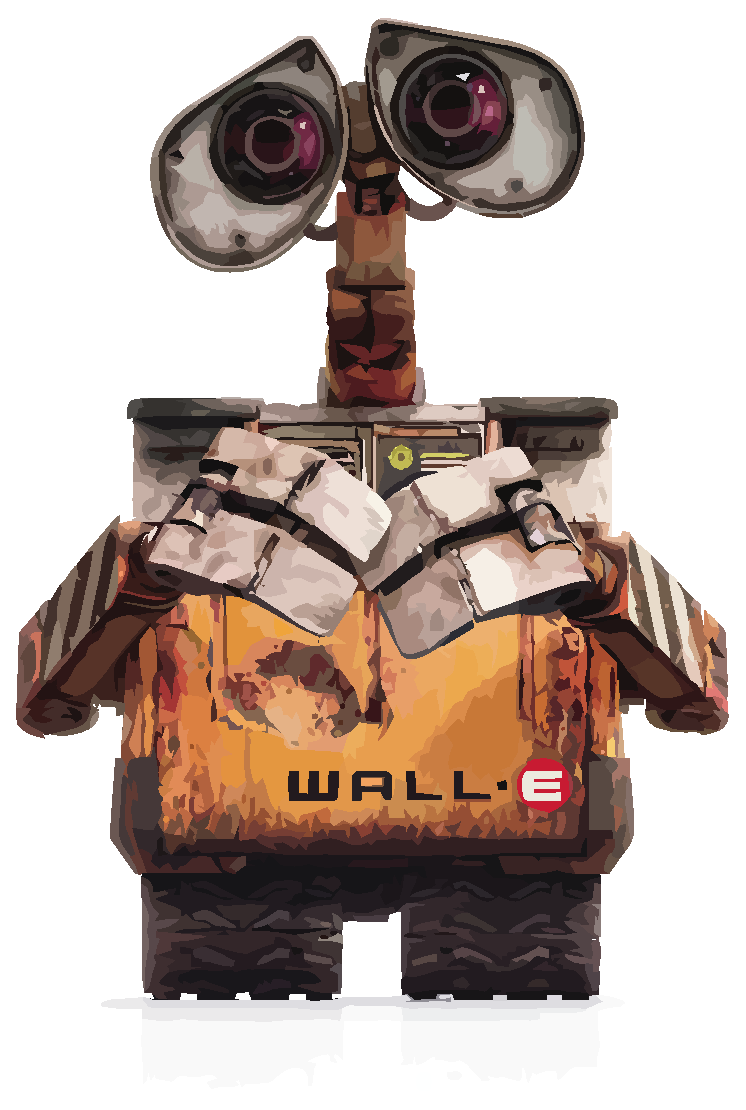
\includegraphics[width=\textwidth]{WallE}
    \caption{Wall-E}
    \label{fig:WallE}
  \end{subfigure}
  \begin{subfigure}[b]{0.3\textwidth}
    
\includegraphics[width=\textwidth]{minion}
    \caption{Minions}
    \label{fig:Minnion}
  \end{subfigure}
  \caption{Best Animations}
  \label{fig:animations}
\end{figure}


\end{landscape}

%!TEX root = ../thesis.tex
%*******************************************************************************
%****************************** Sixth Chapter *********************************
%*******************************************************************************
\graphicspath{{Chapter6/Figs/Vector/}{Chapter6/Figs/}}

%%%%%%%%%%%%%%%%%%%%%%%%%%%%%%%%%%%%%%%%%%%%%%%%%%%%%%%%%%%%%%%%%%%%%%%%%%%%%%%%
% Realization
%%%%%%%%%%%%%%%%%%%%%%%%%%%%%%%%%%%%%%%%%%%%%%%%%%%%%%%%%%%%%%%%%%%%%%%%%%%%%%%%
%
\chapter{Realization}
\section{Introduction}
During the second phase, issues from the backlog were implemented in an iterative SCRUM process. In this chapter, the final realization of the project is evaluated. Findings and observations by considering the assumptions and limitations are discussed. During development, two main applications were written. The price calculation system, and the portal that enables users to manage pricing rules in the price calculation system.

%%%%%%%%%%%%%%%%%%%%%%%%%%%%%%%%%%%%%%%%%%%%%%%%%%%%%%%%%%%%%%%%%%%%%%%%%%%%%%%%
% Sprint 1 - Dynamic Price Calculations
%%%%%%%%%%%%%%%%%%%%%%%%%%%%%%%%%%%%%%%%%%%%%%%%%%%%%%%%%%%%%%%%%%%%%%%%%%%%%%%%
%
\section{Sprint 1 - Dynamic Price Calculations}
A basic dynamic price calculation system was implemented in the first sprint, aiming to deliver a first version of the price calculation system, including fake data generators, validation of models, a single service to determine the distance and duration of a ride, rules that contain pricing information, a calculation that produces the total price of a ride using a companies rules, a formatter that produces an expected response, and tests for all of the functionalities. See Appendix \ref{appendix:slides_1} for the sprint review. Before the beginning of the sprint, different techniques and project structures have been tried, providing a head start.

%%%%%%%%%%%%%%%%%%%%%%%%%%%%%%%%%%%%%%%%%%%%%%%%%%%%%%%%%%%%%%%%%%%%%%%%%%%%%%%%
% Sprint 2 - Authentication and Authorization
%%%%%%%%%%%%%%%%%%%%%%%%%%%%%%%%%%%%%%%%%%%%%%%%%%%%%%%%%%%%%%%%%%%%%%%%%%%%%%%%
%
\section{Sprint 2 - Authentication and Authorization}
Company pricing rules can be used by applications so that each application uses a subset of the pricing rules. For this reason, TPS requires two identifiers to make a price calculation using rules for a particular company application: a companyId and a daAppInstallId. In Appendix \ref{appendix:slides_2_authentication} a proposal has been made to solve authentication for TPS. Authentication has been implemented in this sprint using JSON Web Tokens that are signed by the core system. This implementation saves a lot of maintenance for TPS and other projects that adopt this token format in the future. The token stores two important identifiers that are structurally used in taxiId projects: companyId and daAppInstallId. Companies have one country assigned by default, which determines the currency and VAT percentage. In the breakdown, the VAT percentage is calculated from the actual price, as VAT is included. Discounts are part of the breakdown, being a percentage of the route price, or a fixed price. Another proposal was made to format the breakdown correctly, as shown in Appendix \ref{appendix:slides_2_breakdown}. On top of that, it is possible that a company application uses rules that are related to a debtor, instead of its own subset of rules. These basic steps have been implemented during this sprint, as shown in the sprint review Appendix \ref{appendix:slides_2}. Finally, the project is deployed to a staging environment so that the system could be used by the applications in the staging environment for testing.

%%%%%%%%%%%%%%%%%%%%%%%%%%%%%%%%%%%%%%%%%%%%%%%%%%%%%%%%%%%%%%%%%%%%%%%%%%%%%%%%
% Sprint 3 - Products and Pricing
%%%%%%%%%%%%%%%%%%%%%%%%%%%%%%%%%%%%%%%%%%%%%%%%%%%%%%%%%%%%%%%%%%%%%%%%%%%%%%%%
%
\section{Sprint 3 - Products and Pricing}
At this point the system is fully operational, but company and daAppInstall information has to be inserted in the database manually. An endpoint is made that inserts a full company setup into the database so that prices can be calculated with five products by default. No wireframes were made beforehand, adding to the preliminary tasks of setting up the portal project. Angular in conjunction with Covalents UI platform is used to make the user interface, consisting of an overview and detail page for products and pricing rules. The pricing rules overview shows pricing information for each product that a company has. Whenever a product is added, the pricing information for that new project is automatically added to each rule. Conversely, whenever a new rule is added, all the existing products get their pricing information added to the new rule. On top of that, threshold rules can be added or deleted for distances and durations, making this particular view very complex. This final task is only operational in the backend, so the task of displaying thresholds in the frontend is moved to the next sprint. Appendix \ref{appendix:slides_3} shows some screenshots of the earlier implementations.

%%%%%%%%%%%%%%%%%%%%%%%%%%%%%%%%%%%%%%%%%%%%%%%%%%%%%%%%%%%%%%%%%%%%%%%%%%%%%%%%
% Sprint 4 - Apps and Timeframes
%%%%%%%%%%%%%%%%%%%%%%%%%%%%%%%%%%%%%%%%%%%%%%%%%%%%%%%%%%%%%%%%%%%%%%%%%%%%%%%%
%
\section{Sprint 4 - Apps and Timeframes}
Feedback is given by the product owner after each sprint, resulting in new requirements and modifications to requirements. A functionality is desired that enables users to sort pricing rules and special rates, by dragging the rows in a table to the correct positions. Whenever a priority changes, all subsequent rows need to be updated in order to maintain a consistent prioritized list without duplicate priorities. Another requirement will enable products to be returned in the breakdown as 'on-meter' results. This means that, whenever a destination or departure location is undefined, the system will return products without a price, so that the apps can assign a price later, but will still be aware of the available products. A view is added that displays all apps of a company, and a detail page is added in which rules and discounts can be associated with those apps. This detail page is created in three short iterations. All titles, labels and other texts are replaced by references to a localization api for internationalization purposes. Timeframe components are added to multiple views, in which hours per week can be specified between two dates. For this feature, a proposal was made that is shown in Appendix \ref{appendix:slides_4}.

%%%%%%%%%%%%%%%%%%%%%%%%%%%%%%%%%%%%%%%%%%%%%%%%%%%%%%%%%%%%%%%%%%%%%%%%%%%%%%%%
% Sprint 5 - Thresholds
%%%%%%%%%%%%%%%%%%%%%%%%%%%%%%%%%%%%%%%%%%%%%%%%%%%%%%%%%%%%%%%%%%%%%%%%%%%%%%%%
%
\section{Sprint 5 - Thresholds}
Thresholds, just like prioritized rules and discounts, should be ordered, as they are independently embedded in multiple price entities that are to be synchronized consistently. A rule has pricing information for every product, and every product has many thresholds. Whenever a threshold property is mutated, every other threshold must be updated as well. Also no duplicates are allowed, and no empty price values are allowed inside the thresholds. Thresholds can independently be removed and added, where in the last case values will be copied from the last to the newly added threshold so that the user will not need to manually insert all values. The timeframes are expanded so that either hours per week are used to determine whether a rule should trigger, or a time should be set to further restrict the begin and end date of the timeframes. Price estimations are added as a setting on all relations between all entities and rules, or discounts. Authentication is implemented in the portal so that a JWT is requested at the core system. The token is stored in localstorage and used to communicate with TPS. The automatic call to generate synchronized company data is enabled for the core system, such that every time a company is created in the core system, it is also created in TPS.

%%%%%%%%%%%%%%%%%%%%%%%%%%%%%%%%%%%%%%%%%%%%%%%%%%%%%%%%%%%%%%%%%%%%%%%%%%%%%%%%
% Sprint 6 - Locations
%%%%%%%%%%%%%%%%%%%%%%%%%%%%%%%%%%%%%%%%%%%%%%%%%%%%%%%%%%%%%%%%%%%%%%%%%%%%%%%%
%
\section{Sprint 6 - Locations}
An overview for locations has been added, showing points and areas. A point could be created by searching for a place in Google Places. An area is a larger, more complex area, that should be imported as a more rich polygon. An implementation using OpenStreetMap was able to import complex locations and plot them on a Google Map. Appendix \ref{appendix:slides_6} shows the distinction between the two import functions. After locations have been imported, the user is able to edit the shapes and properties of the location. Because the OpenStreetMap polygons contain far too many indices, the user is confronted with a shape that would take far too long to modify. For this reason, the OpenStreetMap feature was removed from the project. In exchange, the Google Places service point is used as a basis to draw a polygon around. The size of the polygon that is drawn depends on the viewport that Google Places provides, so that larger areas will import larger polygons. Rule subrules had to be added in the rule detail page, for the user to be able to edit multiple rules at once. This issue was not resolved during this sprint, and was moved to the next sprint.

%%%%%%%%%%%%%%%%%%%%%%%%%%%%%%%%%%%%%%%%%%%%%%%%%%%%%%%%%%%%%%%%%%%%%%%%%%%%%%%%
% Sprint 7 - Subrules
%%%%%%%%%%%%%%%%%%%%%%%%%%%%%%%%%%%%%%%%%%%%%%%%%%%%%%%%%%%%%%%%%%%%%%%%%%%%%%%%
%
\section{Sprint 7 - Subrules}
Sub rules were initially estimated to take up two days of development. Each time a sub rule was added, it had to be activated for the same apps as the parent rule. Whenever the parent rule changed its type from 'fixed' to 'dynamic', all sub rules had to be deactivated somehow. Whenever a parent rule ws deleted, all relations had to be deleted in a cascading fashion. And whenever a parent rule's priority changed, the ordering that had to be maintained had to keep the child rules separately updated. This task of micromanaging small properties, keeping data consistent, caused this task to take twice the estimated story points. Appendix \ref{appendix:slides_7} shows the first implementation of subrules. An authorization mixin was added so resources no longer have to be restricted to certain owners manually.

%%%%%%%%%%%%%%%%%%%%%%%%%%%%%%%%%%%%%%%%%%%%%%%%%%%%%%%%%%%%%%%%%%%%%%%%%%%%%%%%
% Sprint 8 - Polishing
%%%%%%%%%%%%%%%%%%%%%%%%%%%%%%%%%%%%%%%%%%%%%%%%%%%%%%%%%%%%%%%%%%%%%%%%%%%%%%%%
%
\section{Sprint 8 - Polishing}
The final major feature changed the way users were able to access predefined locations. An extra tab shows relevant locations defined by taxiID that can be copied and modified in a preview screen. This allows users to set up their locations more quickly. The remaining time is dedicated to fixing bugs and processing feedback.
%!TEX root = ../thesis.tex
%*******************************************************************************
%****************************** Seventh Chapter ********************************
%*******************************************************************************
\graphicspath{{Chapter7/Figs/Vector/}{Chapter7/Figs/}}

%%%%%%%%%%%%%%%%%%%%%%%%%%%%%%%%%%%%%%%%%%%%%%%%%%%%%%%%%%%%%%%%%%%%%%%%%%%%%%%%
% Conclusion
%%%%%%%%%%%%%%%%%%%%%%%%%%%%%%%%%%%%%%%%%%%%%%%%%%%%%%%%%%%%%%%%%%%%%%%%%%%%%%%%
%
\chapter{Conclusion}
\[\textit{How can a generic location-based price calculation system be implemented}\]
\[\textit{that could be used in every country?}\] \hfill

The four challenges manifested in the research questions that constructed this assignment have been answered in order to successfully implement the trip price calculation system. The best possible way of mapping conveyable locations to pricing rules in a system that integrates in the existing system architecture of taxiID, keeping the original rule types while improving the interpretability of the matching logic through the user interface, has been researched. Information available in the public domain has been used to answer empirical questions, from which proposals based on good arguments have been made, and working proof of concepts have been created, out of which some have been implemented, resulting in a system design that could be used for many other purposes in the software industry.


% Locations
Which location encoding is sufficient for this system to be operational?
How can legacy location definitions be improved to be universally interpretable?
In what way can location matching be improved?
Which Database Management Systems are candidate for handling this project's use cases?

Addresses and postal codes can be translated to geometric datatypes such as Points, Polygons and MultiPolygons. Geometry based locations can be visualized, and thus interpreted regardless of the country in which a location resides. Matching is done through the OpenGIS or GeoJSON API, by writing geospatial queries depending on the selected candidate database system. Selected candidate database systems are systems that adhere to the OpenGIS or GeoJSON standard, yielding many possibilities, of which MySQL and MongoDB have been proven to be workable. The problem of overlapping locations, can be solved using complex and straight forward approaches, thus proving this location encoding to be sufficient for this system to be operational.

% Architecture
What is most fitting solution to integrate the backend and frontend into the existing architecture?
Which architectural patterns fit in with the existing system architecture?
How is state shared and synchronized between system components?
What is the most applicable authentication method?

A NodeJS loopback microservice should be implemented along with a MongoDB database, resulting in a scalable high performance solution that can be deployed independently. Introducing a stateless authentication service to implement identity management, allowing the microservice to be more decoupled, bringing the amount of verification requests down to zero. This solution is most fitting to the existing architecture, that only has to implement one future proof authentication method.

% TPS
Which logic and data is required in the backend to reliably calculate a trip price?
Which criteria should regulate whether rules match?
How can determinism of price computations be guaranteed?
In what way can the three original pricing rule types be implemented? (fixed, dynamic, and threshold prices)

Locations should only be used as criteria if the relevant location coordinates are provided by the booking app. Timeframes, passenger count, vehicle types, on-meter and estimation options always apply as criteria by which a rule is matched. The original rules are implemented to each have their own classes, producing deterministic higher order functions that calculate the final trip price, using functional programming techniques.


% Portal
Is it possible to communicate the inner workings of the system through the user interface?
Which backend concepts are essential to display in the frontend?
Which design practices allow users to understand coherence of different elements that make up a rule?
How should a user know what the outcome of his interactions with the system are?

The sidebar reflects which major concepts exist within the portal: Products, Pricing, Locations, and Apps. Composite views reflect the coherence that exists between related entities, while separation of independent entities reduce the cognitive overhead while reasoning about pricing rules. Spatial grouping on the page hint which properties belong to which entity, for which all human beings have a natural intuition. Manual activation and sorting of rules force the user to actively decide whether a rule should match, which can be tested immediately using the companies' booking app.

% ********************************** Back Matter *******************************
% Backmatter should be commented out, if you are using appendices after References
%\backmatter

% ********************************** Bibliography ******************************
\begin{spacing}{0.9}

	% To use the conventional natbib style referencing
	% Bibliography style previews: http://nodonn.tipido.net/bibstyle.php
	% Reference styles: http://sites.stat.psu.edu/~surajit/present/bib.htm

	\bibliographystyle{IEEEtran}
	%\bibliographystyle{unsrt} % Use for unsorted references
	%\bibliographystyle{plainnat} % use this to have URLs listed in References
	\cleardoublepage
	\bibliography{References/references} % Path to your References.bib file


	% If you would like to use BibLaTeX for your references, pass `custombib' as
	% an option in the document class. The location of 'reference.bib' should be
	% specified in the preamble.tex file in the custombib section.
	% Comment out the lines related to natbib above and uncomment the following line.

	%\printbibliography[heading=bibintoc, title={References}]

\end{spacing}

\listoffigures

\listoftables

% ********************************** Appendices ********************************

\begin{appendices} % Using appendices environment for more functionality

	%!TEX root = ../thesis.tex
% ******************************* Thesis Appendix A ****************************
\chapter{Pregame}

\section*{Pregame}
\label{appendix:pregame}

\subsection*{TeXLive package - full version}
\begin{enumerate}
\item	Download the TeXLive ISO (2.2GB) from\\
\href{https://www.tug.org/texlive/}{https://www.tug.org/texlive/}
\item	Download WinCDEmu (if you don't have a virtual drive) from \\
\href{http://wincdemu.sysprogs.org/download/}
{http://wincdemu.sysprogs.org/download/}
\item	To install Windows CD Emulator follow the instructions at\\
\href{http://wincdemu.sysprogs.org/tutorials/install/}
{http://wincdemu.sysprogs.org/tutorials/install/}
\item	Right click the iso and mount it using the WinCDEmu as shown in \\
\href{http://wincdemu.sysprogs.org/tutorials/mount/}{
http://wincdemu.sysprogs.org/tutorials/mount/}
\item	Open your virtual drive and run setup.pl
\end{enumerate}

or

\subsection*{Basic MikTeX - \TeX~ distribution}
\begin{enumerate}
\item	Download Basic-MiK\TeX (32bit or 64bit) from\\
\href{http://miktex.org/download}{http://miktex.org/download}
\item	Run the installer
\item	To add a new package go to Start >> All Programs >> MikTex >> Maintenance (Admin) and choose Package Manager
\item	Select or search for packages to install
\end{enumerate}

\subsection*{TexStudio - \TeX~ editor}
\begin{enumerate}
\item	Download TexStudio from\\
\href{http://texstudio.sourceforge.net/\#downloads}
{http://texstudio.sourceforge.net/\#downloads}
\item	Run the installer
\end{enumerate}

\section*{Mac OS X}
\subsection*{MacTeX - \TeX~ distribution}
\begin{enumerate}
\item	Download the file from\\
\href{https://www.tug.org/mactex/}{https://www.tug.org/mactex/}
\item	Extract and double click to run the installer. It does the entire configuration, sit back and relax.
\end{enumerate}

\subsection*{TexStudio - \TeX~ editor}
\begin{enumerate}
\item	Download TexStudio from\\
\href{http://texstudio.sourceforge.net/\#downloads}
{http://texstudio.sourceforge.net/\#downloads}
\item	Extract and Start
\end{enumerate}


\section*{Unix/Linux}
\subsection*{TeXLive - \TeX~ distribution}
\subsubsection*{Getting the distribution:}
\begin{enumerate}
\item	TexLive can be downloaded from\\
\href{http://www.tug.org/texlive/acquire-netinstall.html}
{http://www.tug.org/texlive/acquire-netinstall.html}.
\item	TexLive is provided by most operating system you can use (rpm,apt-get or yum) to get TexLive distributions
\end{enumerate}

\subsubsection*{Installation}
\begin{enumerate}
\item	Mount the ISO file in the mnt directory
\begin{verbatim}
mount -t iso9660 -o ro,loop,noauto /your/texlive####.iso /mnt
\end{verbatim}

\item	Install wget on your OS (use rpm, apt-get or yum install)
\item	Run the installer script install-tl.
\begin{verbatim}
	cd /your/download/directory
	./install-tl
\end{verbatim}
\item	Enter command `i' for installation

\item	Post-Installation configuration:\\
\href{http://www.tug.org/texlive/doc/texlive-en/texlive-en.html\#x1-320003.4.1}
{http://www.tug.org/texlive/doc/texlive-en/texlive-en.html\#x1-320003.4.1}
\item	Set the path for the directory of TexLive binaries in your .bashrc file
\end{enumerate}

\subsubsection*{For 32bit OS}
For Bourne-compatible shells such as bash, and using Intel x86 GNU/Linux and a default directory setup as an example, the file to edit might be \begin{verbatim}
edit $~/.bashrc file and add following lines
PATH=/usr/local/texlive/2011/bin/i386-linux:$PATH;
export PATH
MANPATH=/usr/local/texlive/2011/texmf/doc/man:$MANPATH;
export MANPATH
INFOPATH=/usr/local/texlive/2011/texmf/doc/info:$INFOPATH;
export INFOPATH
\end{verbatim}
\subsubsection*{For 64bit OS}
\begin{verbatim}
edit $~/.bashrc file and add following lines
PATH=/usr/local/texlive/2011/bin/x86_64-linux:$PATH;
export PATH
MANPATH=/usr/local/texlive/2011/texmf/doc/man:$MANPATH;
export MANPATH
INFOPATH=/usr/local/texlive/2011/texmf/doc/info:$INFOPATH;
export INFOPATH

\end{verbatim}



%\subsection{Installing directly using Linux packages}
\subsubsection*{Fedora/RedHat/CentOS:}
\begin{verbatim}
sudo yum install texlive
sudo yum install psutils
\end{verbatim}


\subsubsection*{SUSE:}
\begin{verbatim}
sudo zypper install texlive
\end{verbatim}


\subsubsection*{Debian/Ubuntu:}
\begin{verbatim}
sudo apt-get install texlive texlive-latex-extra
sudo apt-get install psutils
\end{verbatim}

	%!TEX root = ../thesis.tex
% ******************************* Thesis Appendix B ****************************
\graphicspath{{Appendix2/Figs/Vector/}{Appendix2/Figs/}}

\chapter{Sprint Summaries}

\section*{Sprint Summaries}
\label{appendix:sprints}

% \begin{figure}[htbp!]
% 	\centering
% 	
\includegraphics[width=1\textwidth]{DriveFolder}
% 	\label{fig:Folder}
% \end{figure}

\url{https://goo.gl/BR75HN}

\end{appendices}

% *************************************** Index ********************************
\printthesisindex % If index is present

\end{document}
